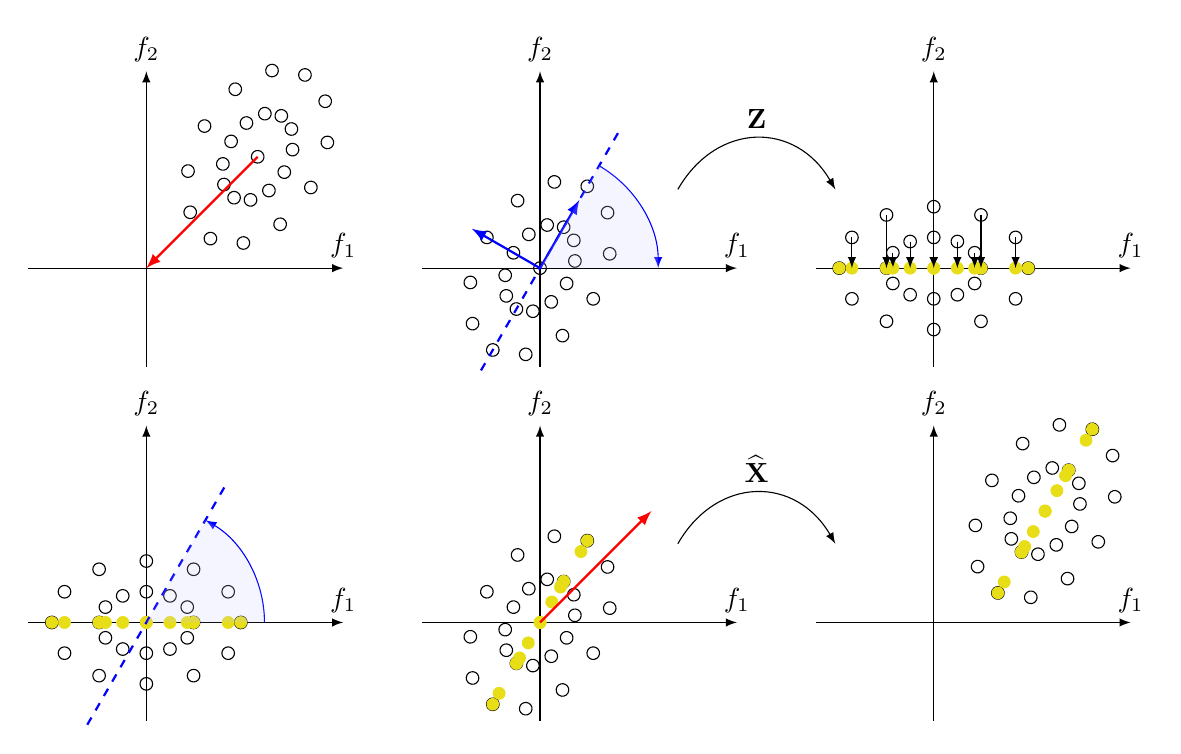
\begin{tikzpicture}[> = latex]

    \def\r{0.08}
    \def\drawAxis{
        \draw [->] (-1.5, 0) -- (2.5, 0) node [above] {$f_1$};
        \draw [->] (0, -1.25) -- (0, 2.5) node [above] {$f_2$};
    }
    \def\drawEllipticalData{
        \draw (0, 0) circle (\r);
        \foreach \mag in {0.6, 1.2}{
            \foreach \ang in {0, 30,..., 330}{
                \draw ({\mag * cos(\ang)}, {0.65 * \mag * sin(\ang)}) circle (\r);
            }
        }
    }
    \def\drawProjections{
        \fill [yellow!90!black] (0, 0) circle (\r);
        \foreach \mag in {0.6, 1.2}{
            \foreach \ang in {0, 30,..., 330}{
                \draw ({\mag * cos(\ang)}, {0.65 * \mag * sin(\ang)}) circle (\r);
                \fill [yellow!90!black] ({\mag * cos(\ang)}, 0) circle (\r);
            }
            \foreach \ang in {30, 60, ..., 150}{
                \draw [->] ({\mag * cos(\ang)}, {0.65 * \mag * sin(\ang)}) -- ({\mag * cos(\ang)}, 0);
            }
        }
    }
    \def\drawProjectionsNoArrows{
        \fill [yellow!90!black] (0, 0) circle (\r);
        \foreach \mag in {0.6, 1.2}{
            \foreach \ang in {0, 30,..., 330}{
                \draw ({\mag * cos(\ang)}, {0.65 * \mag * sin(\ang)}) circle (\r);
                \fill [yellow!90!black] ({\mag * cos(\ang)}, 0) circle (\r);
            }
        }
    }

    % Original data
    \drawAxis
    \begin{scope}[shift={(45:2)}, rotate=60]
        \drawEllipticalData
    \end{scope}
    % Centroid
    \draw [->, thick, red] (45:2) -- (0:0);

    % Zero mean data
    \begin{scope}[shift={(5, 0)}]
        \drawAxis
        \begin{scope}[rotate=60]
            \drawEllipticalData
        \end{scope}
        % Orthonormal eigenvectors
        \draw [dashed, thick, blue] (60:-1.5) -- (60:2); % direction of v1
        \draw [->, thick, blue] (0:0) -- (60:1); % v1
        \draw [->, thick, blue] (0:0) -- (60+90:1); % v2

        % Rotation
        \draw [->, blue] (60:1.5) arc (60:0:1.5);
        \fill [blue!20, opacity=0.2]
            (0:0) -- (60:1.5) arc (60:0:1.5) -- cycle
        ;
    \end{scope}

    \draw [->] 
        (6.75, 1) .. controls ++(60:1) and ++(120:1) .. (8.75, 1) 
        node [midway, above] {$\mathbf{Z}$}
    ;

    % Projections onto biggest eigenvector
    \begin{scope}[shift={(10, 0)}]
        \drawAxis
        % \drawEllipticalData

        % Projections
        \drawProjections
    \end{scope}

    % Reconstructions: rotation
    \begin{scope}[shift={(0, -4.5)}]
        \drawAxis
        % \drawEllipticalData

        % Projections
        \drawProjectionsNoArrows

        % Orthonormal eigenvectors
        \draw [dashed, thick, blue] (60:-1.5) -- (60:2); % direction of v1

        % Rotation
        \draw [<-, blue] (60:1.5) arc (60:0:1.5);
        \fill [blue!20, opacity=0.2]
            (0:0) -- (60:1.5) arc (60:0:1.5) -- cycle
        ;
    \end{scope}

    % Reconstructions: translation
    \begin{scope}[shift={(5, -4.5)}]
        \drawAxis

        \begin{scope}[rotate=60]
            \drawProjectionsNoArrows
        \end{scope}

        \draw [<-, thick, red] (45:2) -- (0:0);
    \end{scope}

    \draw [->] 
        (6.75, 1-4.5) .. controls ++(60:1) and ++(120:1) .. (8.75, 1-4.5) 
        node [midway, above] {$\widehat{\mathbf{X}}$}
    ;

    % Reconstructions: results
    \begin{scope}[shift={(10, -4.5)}]
        \drawAxis

        \begin{scope}[shift={(45:2)}, rotate=60]
            \drawProjectionsNoArrows
        \end{scope}
    \end{scope}
\end{tikzpicture}